\section{Results}

To test the clustering algorithm, a terrain is loaded, it's resources edited and five clusters produced. These clusters are subsequently analysed to ensure they successfully detect distinct resource features on which to cluster.\\

The terrain used is a model of the Grand Canyon using data from the US Geological Survey \protect\footnotemark \footnotetext{\url{http://www.usgs.gov}}. This terrain is chosen as its canyons and crevasses make ground illumination vary greatly.\\

The following resource edits were performed on the terrain:

\begin{itemize}
\item \textit{Latitude}: Set to zero degrees (equator)
\item \textit{Soil Infiltration}: 5 millimetres for all terrain points with a slope under 30 degrees. All points with a slope over 30 degrees were set to 0 to simulate a cliff.
\item \textit{Rainfall}: See table \ref{tab:clustering_test_rainfall}.
\item \textit{Temperature}: 0 degrees at 0 meters in December. 15 degrees at 0 metres in June. Lapse rate at default value of 6.4 degrees per thousand metres.
\end{itemize}

The resulting terrain clusters that form are displayed in figure \ref{fig:clustering_test_resulting_clusters} and summarized in appendix \ref{AppendixA}.

\begin{table}[]
  \centering
	    \begin{tabular}{|p{5cm}|p{5cm}|}
	    \hline
	    \textbf{Month} & \textbf{Rainfall (mm)}\\
		\hline
	    Jan & 13 \\
	    \hline
	    Feb & 15 \\
	    \hline
	    Mar & 14 \\
	    \hline
	    Apr & 9 \\
	    \hline
	    May & 6 \\
	    \hline
	    Jun & 18 \\
	    \hline
	    Jul & 18 \\
	    \hline
	    Aug & 22 \\
	    \hline
	    Sep & 15 \\
	    \hline
	    Oct & 11 \\
	    \hline
	    Nov & 9 \\
	    \hline
	    Dec & 16 \\
	    \hline
		\end{tabular}
		\caption{Monthly rainfall configured for the clustering tests.}
	  \label{tab:clustering_test_rainfall}
\end{table}

\begin{figure}
\center
	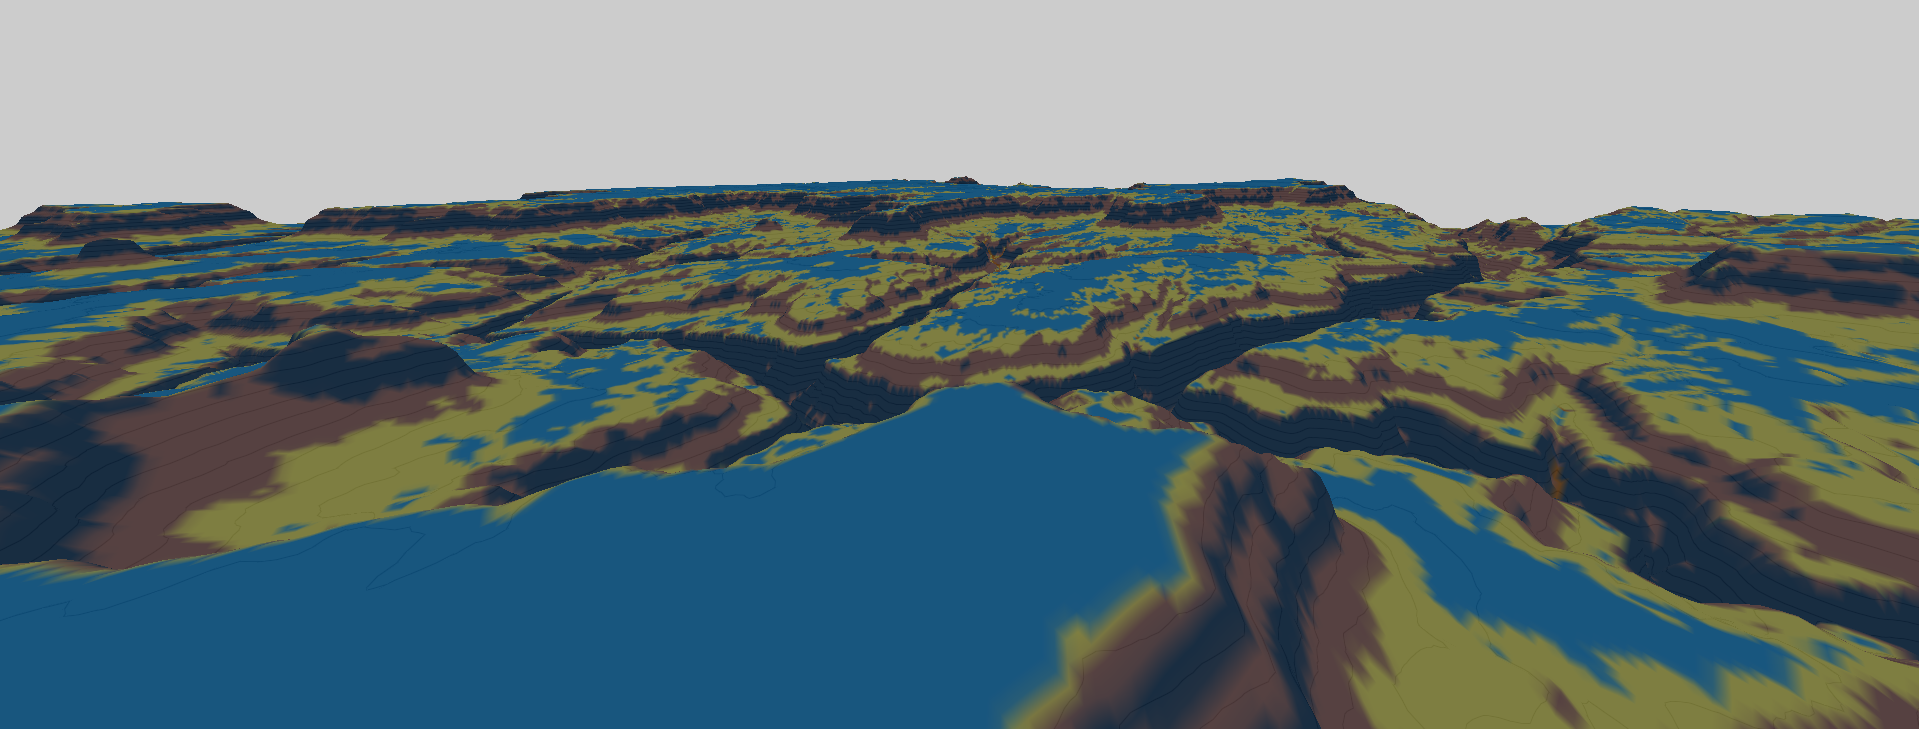
\includegraphics[width=\textwidth]{clustering_test_resulting_clusters.png}
	\caption{ \textit{Clustering test: Resulting terrain clusters}}	
	\label{fig:clustering_test_resulting_clusters}
\end{figure}

\begin{figure}
\center
	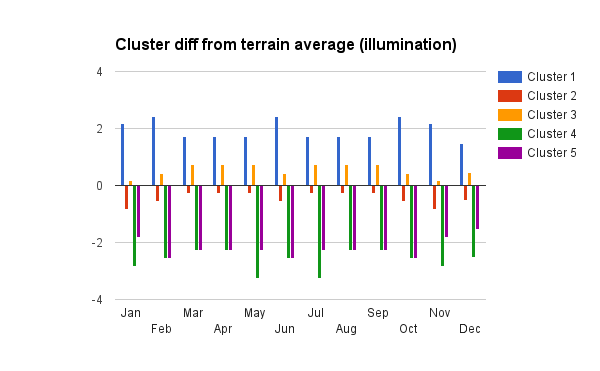
\includegraphics[width=\textwidth]{clustering_graph_illumination_diff.png}
	\caption{ \textit{Monthly illumination for each cluster and the average over the whole terrain.}}	
	\label{fig:clustering_graph_illumination}
\end{figure}

\begin{figure}
\center
	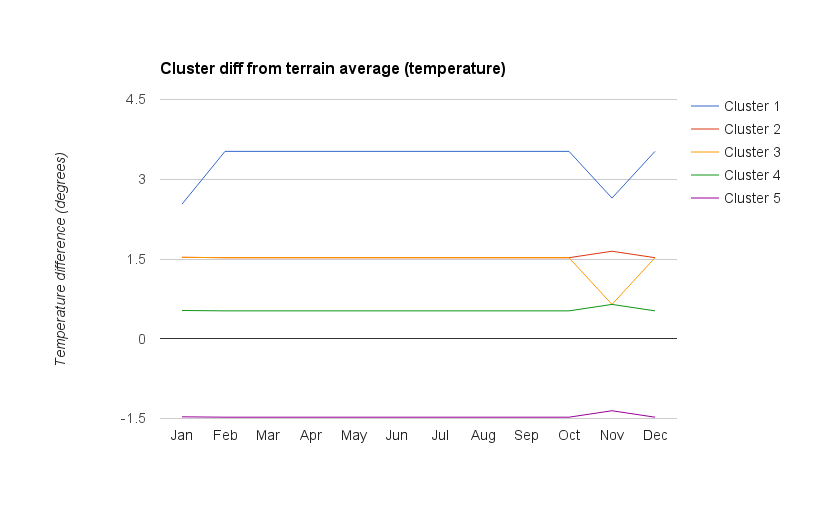
\includegraphics[width=\textwidth]{clustering_graph_temp_diff.png}
	\caption{ \textit{Monthly temperature for each cluster and the average over the whole terrain. Cluster 2 has the same values as cluster 4.}}	
	\label{fig:clustering_graph_temp}
\end{figure}

\begin{figure}
\center
	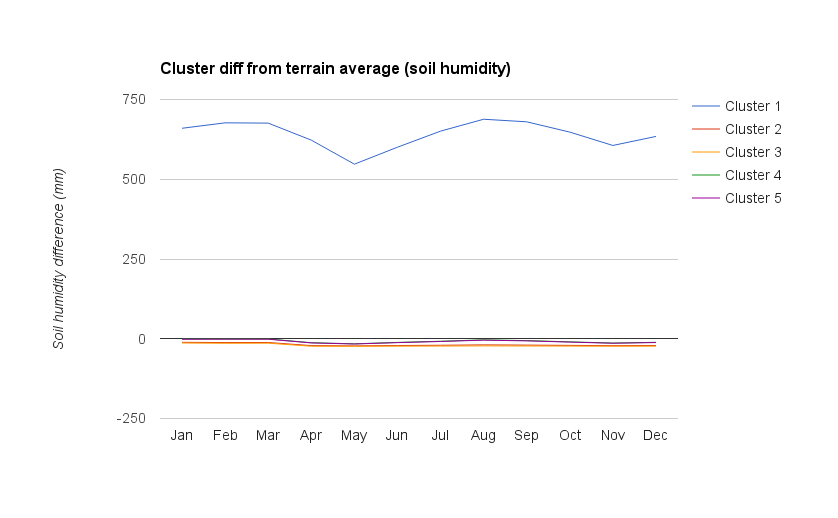
\includegraphics[width=\textwidth]{clustering_graph_soil_humidity_diff.png}
	\caption{ \textit{Soil humidity for each cluster (same for every month) and the average over the whole terrain.}}	
	\label{fig:clustering_graph_humidity}
\end{figure}

\begin{table}[]
  \centering
	\begin{tabular}{|p{5cm}|p{5cm}|}
	\hline
	\textbf{Cluster ID} & \textbf{Slope difference (degrees)}\\
	\hline
	1 & -2.5 \\	
	\hline
	2 & 36.7\\	
	\hline
	3 & 59.5\\	
	\hline
	4 & -18\\	
	\hline
	5 & -53.5\\		
	\hline
	\end{tabular}
	\caption{ Difference of slope between the means of each cluster and the terrain mean.}
	\label{tab:clustering_slope_mean}
\end{table}

Figures \ref{fig:clustering_graph_illumination}, \ref{fig:clustering_graph_temp}, \ref{fig:clustering_graph_humidity} and table \ref{tab:clustering_slope_mean} show how much each cluster's illumination, temperature, soil humidity and slope vary from the terrain's average.\\ 

From figure \ref{tab:clustering_test_cluster_variance}, which summarises the resource variance of each cluster, it is possible to identify key terrain features the represent, notably: \textit{Cluster 1} is formed of the data points within the flat bottom of the canyon where the rivers form. Hence the low temperature caused by the low altitude, the low illumination caused by the surrounding canyon walls casting shade, the extremely high humidity caused by the river stream passing through and the flat bottom causing the slope to be very low. \textit{Cluster 2} constitutes the points at the top of the canyon cliffs where slope reduces. Hence the high slope and the low humidity (water run-off). \textit{Cluster 3} contains the data points on the cliffs of the terrain, hence the high slopes, low humidity (water run-off) and low illumination (cliffs often in the shade). \textit{Cluster 4} is formed of the data points most similar to the terrain mean, hence its limited variance. \textit{Cluster 5} is formed of the areas of high altitudes where the surface is flat, illumination is high (nothing to shade it) and temperatures are low.\\

\begin{table}[]
  \centering
	    \begin{tabular}{|p{3cm}|p{3cm}|p{3cm}|p{3cm}|p{3cm}|}
		\hline	
  	    \textbf{Cluster} &  \textbf{Illumination} & \textbf{Temperature} & \textbf{Soil Humidity} & \textbf{Slope} \\
		\hline
		\textbf{1} & 4(-) & 5(+)$^{*}$ & 5(+)$^{*}$ & 1(-) \\
		\hline
		\textbf{2} & 2(-) & 4(+) & 3(-) & 3(+) \\
		\hline
		\textbf{3} & 5(-)$^{*}$ & 2(+) & 4(-)$^{*}$ & 5(+)$^{*}$ \\
		\hline
		\textbf{4} & 1(+) & 1(+) & 1(-) & 2(-) \\
		\hline
		\textbf{5} & 3(+)$^{*}$ & 3(-)$^{*}$ & 2(-) & 4(-)$^{*}$ \\
		\hline
		\end{tabular}
		\caption{Comparison of cluster feature variance from terrain average on a ranking of 1 (least) to 5 (most). The symbol states whether the variance is positive (+) or negative (-). The minimums and maximums for each resource are represented with a $^{*}$. }
	  \label{tab:clustering_test_cluster_variance}
\end{table}